\chapter{Experiments and Clinical Test}
This Chapter explains the setup for testing the basic device functionalities. The Chapter also discusses the clinical test conducted at LaBioMed at Torrance using Mannequin-based Patient Simulation. The study protocol, analysis and preliminary results will be discussed.

\section{Motivation}
The motivation for the study can be broken down into the following
\begin{itemize}
	\item To perform preliminary testing of device functionalities and to test if the system runtime requirement is fulfilled
	
	\item To perform a clinical test to evaluate the signal quality and to test the usability
	
	\item To obtain suite of signals in a data set for future algorithm optimization
	 
\end{itemize}

\section{Preliminary Experiments and System Characterization}
\subsection{Setup}
The basic device functionality of the device is tested by simulating the required signals locally in our lab. The ECG signal is simulated using Precise Life SKX 2000 ECG simulator(Figure \ref{fig:ecg_sim}). The ECG is interfaced in 4 lead configuration using right arm(RA), left arm(LA), left leg(LL) and right leg(RL) drive leads. 
\begin{figure}[h]
	\centering
	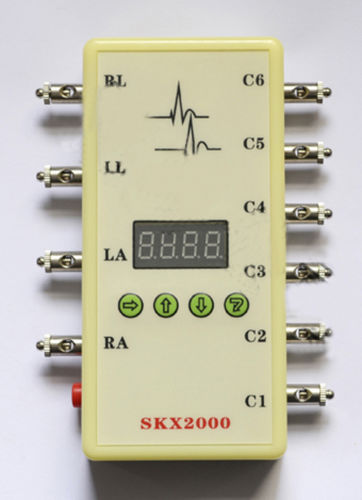
\includegraphics[scale = 0.5 ]{ecg_sim.JPG}
	\caption{ECG Simulator\label{fig:ecg_sim}}
\end{figure}

 The body temperature is simulated using sodium acetate based reusable head pods. The acceleration of chest, paramedic log and breathing sound are manually simulated.

The system is tested with the firmware that incorporated the techniques mentioned in the previous chapter. 
In order to determine the  power dissipation, the relative contribution of the different parts of the system needs to be considered.  First, the idle mode current of the system was measured to be 22 mA.The environment temperature sensor, ECG front end chip and the accelerometer are  powered directly from the battery. They are not controlled by the DSP, so the state of the DSP does not affect their power consumption.These components contribute to idle mode current consumption. Then the average current of the system with all the sensors and DSP (running at 100MHz) being active was measured to be 38.64 mA. The average current drawn when writing to the SD card while all the components of the system are active was measured to be 48 mA. The current drawn by the system was measured using INA231 evaluation module, which samples the current drawn by the system  every 140 uS and logs the data.This data was used for the calculation.
\begin{table}[h]
	\centering
	\begin{tabular}{|l|l|}
		\hline
		$Operation$ & $Current$\\
		\hline
		Idle &  22 mA\\
		Data Acquisition &  38.64\\
		Micro SD write & 48 mA \\
		\hline
	\end{tabular}
	\caption{Current drawn for different operation mode.}
	\label{table:ecg}
\end{table}

The BlueBox was tested for different time duration ranging from 15 mins to 3 hours. The average current consumption of the system during the test was measured to be approximately 50 mA. With this rate the system should be able to run for 5-6 hours .

The acquired data was verfied by primarily reconstructing the signal and confirm if the amount of samples of each signal is equivalent to the test duration. This ensures the correctness of the process of data recording. The validity of the data was verified manually from playing back the signals and validating if the reflected the conditions during the test.
\section{Clinical test setup and protocol}

\subsection{Mannequin-based Patient Simulation}
BlueBox initial clinical test is done with a Mannequin-based patient simulation environment.
Taking the underlying concepts described for the desktop simulation one step further is the recreation of the real physical patient in a realistic physical clinical environment \cite{man}. Thus, computerized mannequin stands in for the patient, and a variety of equipment can be used (either real clinical equipment or computer-driven replicas) to monitor and treat the patient.
Among the functions that these mannequin-based simulators can replicate are:
\begin{itemize}
	\item Spontaneous breathing (and the ability to breathe for the patient with a bag or ventilator)
	\item Pulses, heart sounds, breath sounds, pupil size, pupil response to light
	
	\item Real-time display of electronically monitored information (e.g. ECG, oxygen saturation, etc.)	
\end{itemize}

Not only are these created in their “normal” manifestation, but all the elements of a large variety of abnormal conditions can be created such as (the list is almost endless) heart attack, severe allergic reaction, breathing difficulties, sepsis (“blood poisoning”), severe abnormalities of sugar metabolism, etc.

\subsection{Test Protocol}
The test was done with the BlueBox device placed on the Mannequin's chest. The Mannequin wore the four electrode model in a lead II configuration. The body temperature sensor is worn near the mannequin's neck.The contact mirophone to record the respiration sound is placed on the mannequin's abdomen. The environment microphone to record paramedic's comments is on the top of the device. As the accelerometer is on board, it can measure the chest rise of the mannequin.The on-board temperature sensor can measure environment temperature.  The preliminary tests were conducted for different time duration ranging from 15 minutes to 2 hours.The tests were conducted under normal conditions and variety of abnormal conditions like heart attack, severe allergic reaction, breathing difficulties etc. The device is switched on using a button during the beginning of th experiment and after the test duration is completed, the data is imported into the computer to verify if the signal reflected the test conditions. The lab researchers and doctors on the IRB are required to be present for the duration of the test. 

\section{Analysis and Result}
\begin{figure}
	\centering
	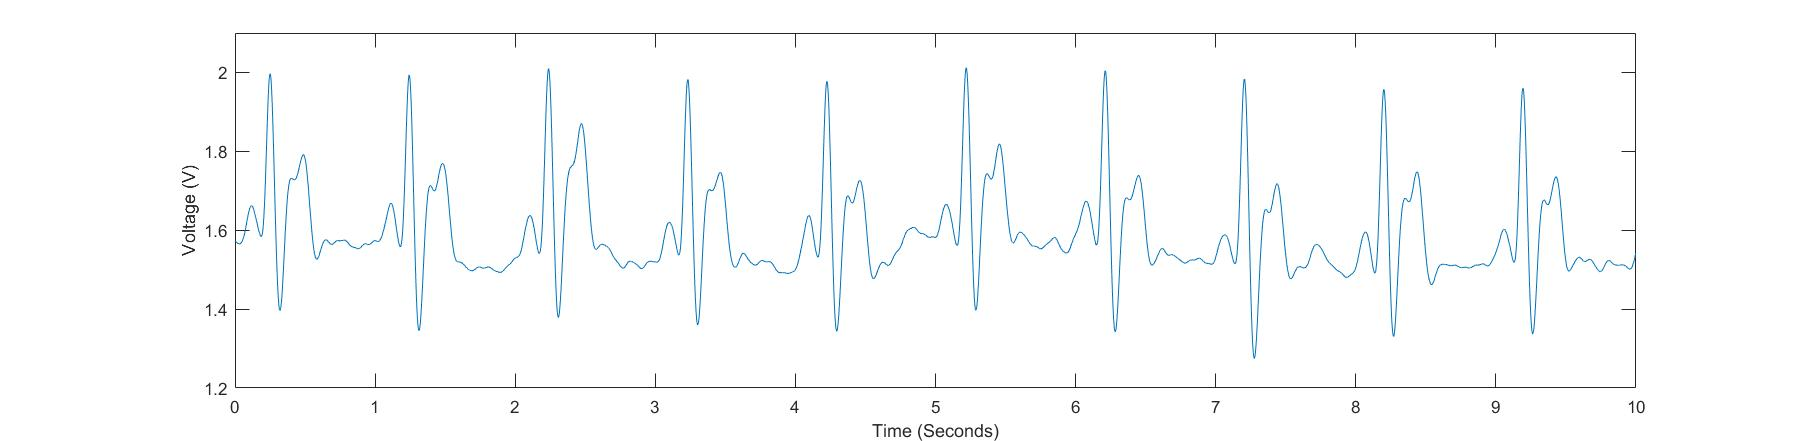
\includegraphics[scale = 0.25 ]{ECG_result.jpg}
	\caption{ECG Signal\label{fig:ecg_res}}
\end{figure}
\begin{figure}[h]
	\centering
	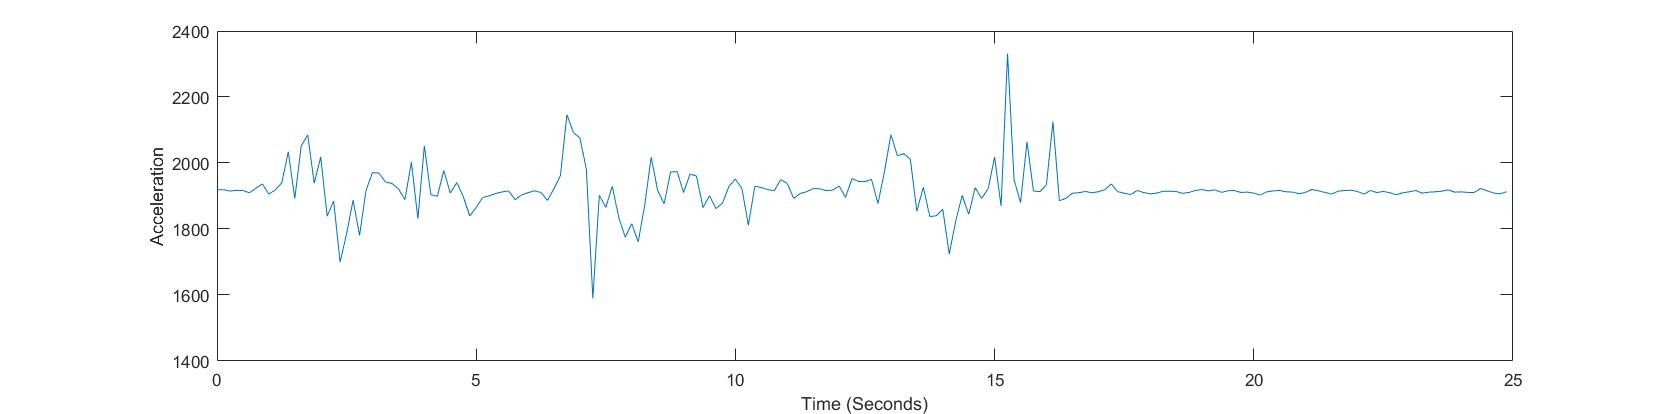
\includegraphics[scale = 0.25 ]{acc_result.jpg}
	\caption{Accelerometer Signal\label{fig:acc_res}}
\end{figure}


The important objective of the test is to evaluate the signal quality and performance of the BlueBox device. This is achieved by comparing the acquired signal with the originally simulated signals. The computerized mannequin has a record of all physically simulated signals (including ECG, breathing pattern and body temperature). All the vitals are compared with the original signal for evaluation. The two ECG signals are aligned in time to make a simple analysis.By analyzing these two signals physicians concluded that the acquired signal is reliable.Body temperature and chest movements were also analyzed with the same manner and are reliable. 
The figures \ref{fig:ecg_res}, \ref{fig:btemp_res},\ref{fig:env_res} \& \ref{fig:acc_res} shows the samples of results of signals measured during the Clinical tests.

\begin{figure}[h]
	\centering
	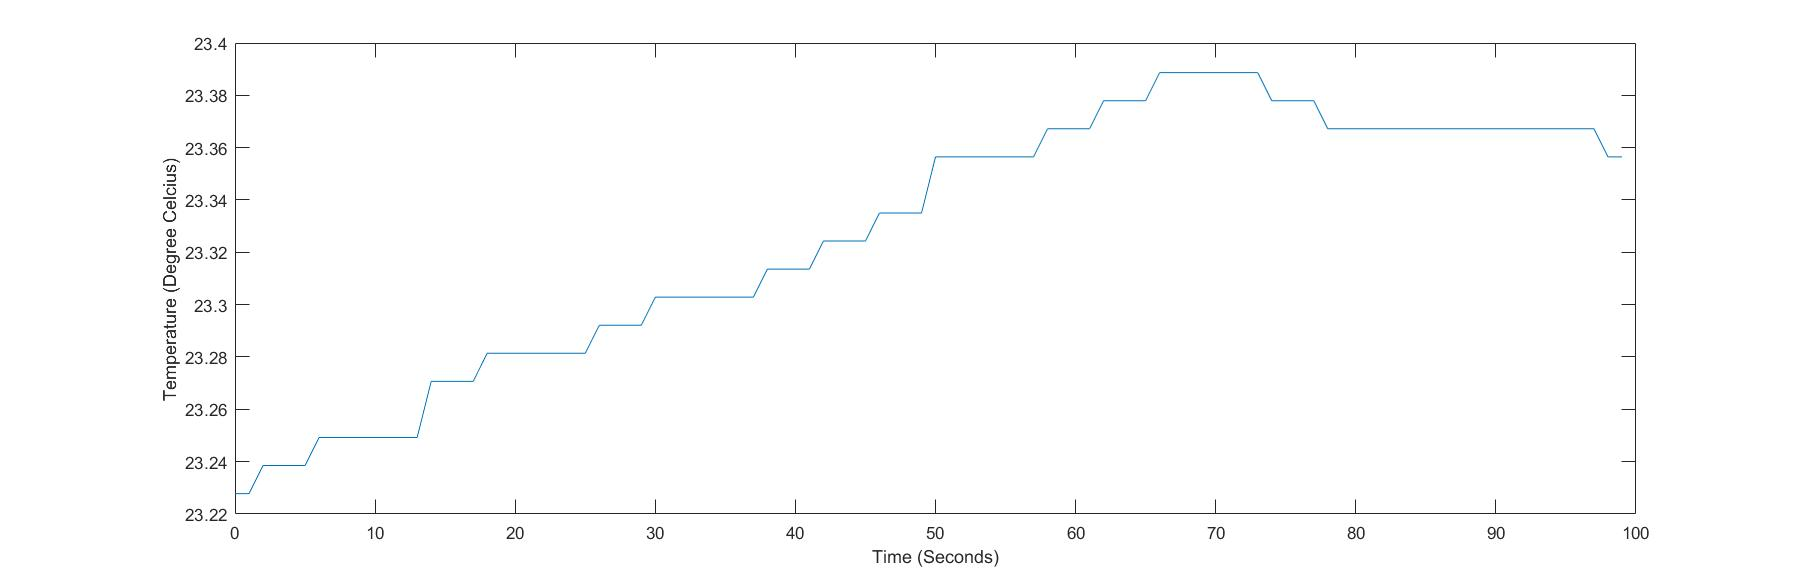
\includegraphics[scale = 0.20 ]{envT_result.jpg}
	\caption{Environment Temperature\label{fig:env_res}}
\end{figure}



\begin{figure}[h]
	\centering
	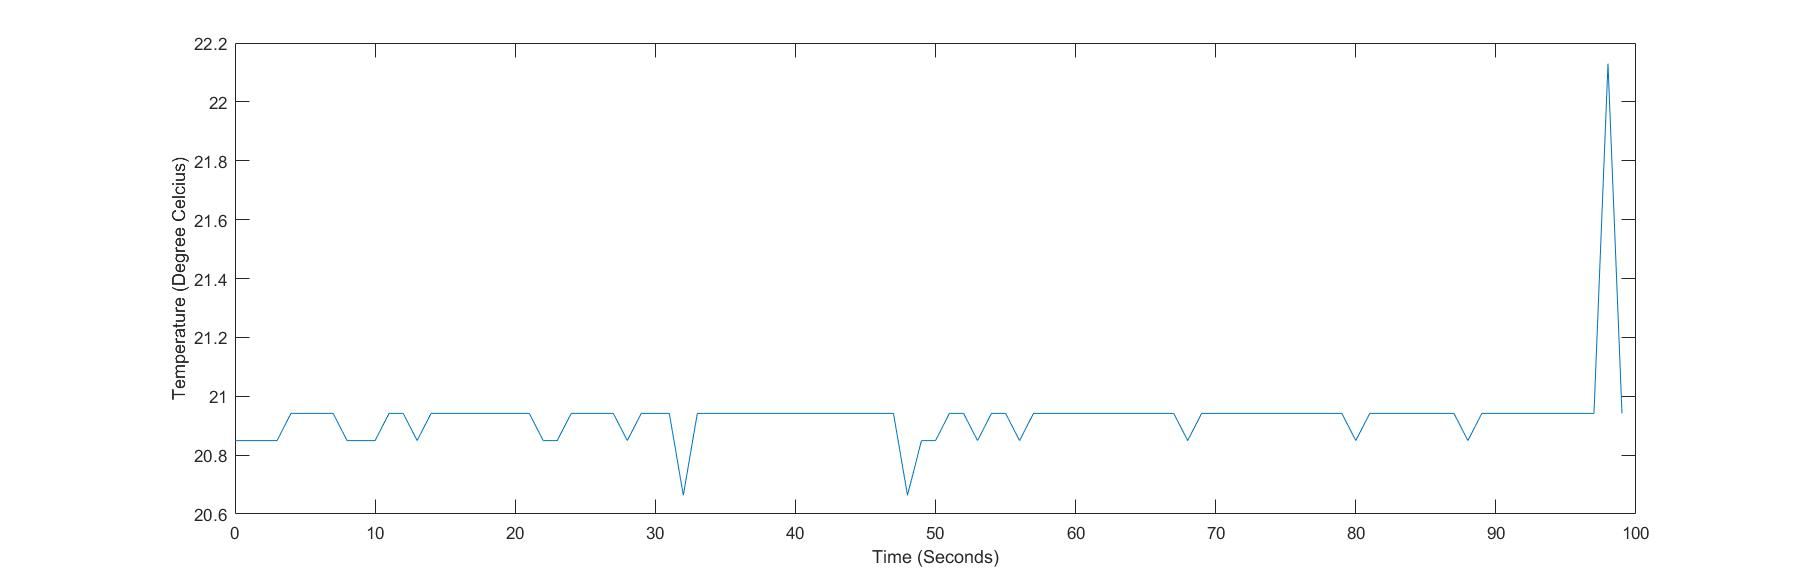
\includegraphics[scale = 0.22 ]{btemp_result.jpg}
	\caption{Body Temperature\label{fig:btemp_res}}
\end{figure}

The environment temperature is evaluated by simultaneously measuring the environment temperature using a standard device and comparing their values. This comparison confirmed the reliability of it. 
The two channels of audio acquired are analyzed by playing it back and manually verifying the quality. The analysis concluded that paramedic's log audio signal carries the required information along with some noise. It requires a proper post processing in order to remove noise. The contact microphone was sensitive to the paramedic's logs and it kind of made the breathing sound feeble. A microphone or a sensor that could be sensitive to the respiration and not sensitive to the atmospheric noise to be developed in order to get the required respiration information.



